\documentclass[10pt, t]{beamer}
\usetheme{metropolis}           % Use metropolis theme

\ifnotes
  \hypersetup{final}
  \usepackage{pgfpages}
  \setbeamertemplate{note page}[plain]
  \setbeameroption{show notes on second screen=right}
  % the following fixes bug which causes normal text to be white instead of
  % template default when notes are enabled
  % (see https://tex.stackexchange.com/questions/232168/normal-text-is-invisible-when-using-beamer-with-notes-and-xelatex)
  \makeatletter 
  \def\beamer@framenotesbegin{% at beginning of slide
       \usebeamercolor[fg]{normal text}
        \gdef\beamer@noteitems{}% 
        \gdef\beamer@notes{}% 
  }
  \makeatother
\fi

\usepackage{appendixnumberbeamer}
\usepackage{multirow}
\usepackage{verbatim}
\usepackage{tikz}
\usetikzlibrary{decorations.pathreplacing}
\usepackage[scale=3]{ccicons}   % creative commons icons

\title{Parallel computing platforms}
\date{}
\author{Jeremy Iverson}
\institute{College of Saint Benedict \& Saint John's University}
\begin{document}
  \maketitle

  \begin{frame}{recap}
    \begin{itemize}
      \item von Neumann architecture
        \begin{itemize}
          \item central processing unit
          \item memory
            \begin{itemize}
              \item cache (\$)
            \end{itemize}
          \item interconnection
        \end{itemize}
      \item operating system
        \begin{itemize}
          \item processes vs threads
        \end{itemize}
    \end{itemize}

    \note{
      \begin{itemize}
        \item \texttt{lscpu}
        \item \texttt{cat /proc/cpuinfo} activity for CPU info
        \item \texttt{cat /sys/devices/system/cpu/cpu0/cache/} for cache info
        \item L1, L2, L3
          \begin{itemize}
            \item L1 is usually split into data and instruction
            \item L2 is usually not shared, i.e., each core has its own
            \item L3 is usually shared by multiple cores
          \end{itemize}
        \item multitasking operating system, runs many processes despite having
          only one or a ``small'' number of physical cores
          \begin{itemize}
            \item context switches the processes at predefined time slices
            \item \texttt{top} activity
          \end{itemize}
        \item generally speaking, processes have their own address space,
          threads share an address space
      \end{itemize}
    }
  \end{frame}

  \begin{frame}[fragile]{cache performance}
    From Intel Performance Analysis Guide:
    \begin{tiny}
      \begin{verbatim}
        Core i7 Xeon 5500 Series Data Source Latency (approximate)               [Pg. 22]

        local  L1 CACHE hit,                              ~4 cycles (   2.1 -  1.2 ns )
        local  L2 CACHE hit,                             ~10 cycles (   5.3 -  3.0 ns )
        local  L3 CACHE hit, line unshared               ~40 cycles (  21.4 - 12.0 ns )
        local  L3 CACHE hit, shared line in another core ~65 cycles (  34.8 - 19.5 ns )
        local  L3 CACHE hit, modified in another core    ~75 cycles (  40.2 - 22.5 ns )

        remote L3 CACHE (Ref: Fig.1 [Pg. 5])        ~100-300 cycles ( 160.7 - 30.0 ns )

        local  DRAM                                                   ~60 ns
        remote DRAM                                                  ~100 ns
      \end{verbatim}
    \end{tiny}
  \end{frame}

  \begin{frame}{cache performance}
    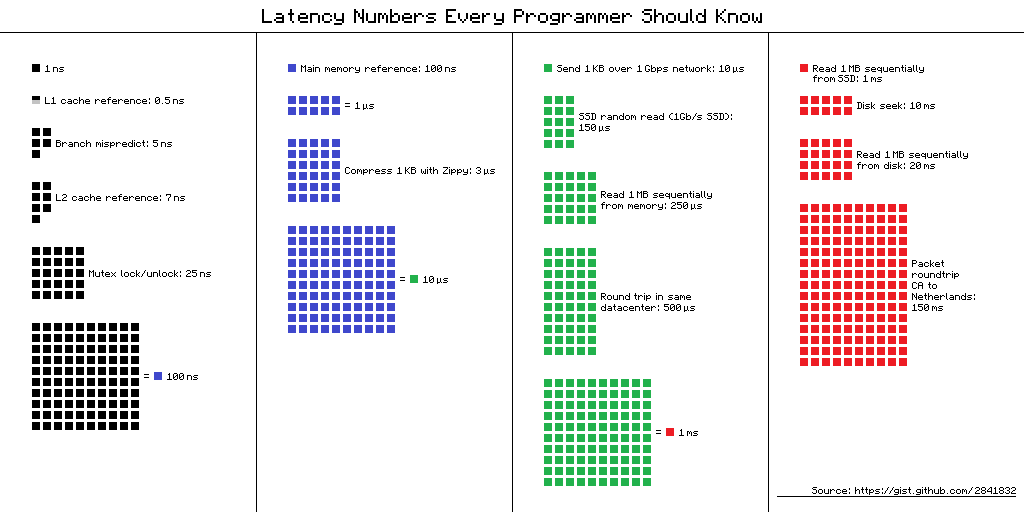
\includegraphics[width=\textwidth]{cache-perf.png}\\
    \hfill \tiny{\href{https://i.stack.imgur.com/a7jWu.png}{Latency Numbers
    Every Programmer Should Know}}
  \end{frame}

  \begin{frame}{parallel computing platform}
    \begin{itemize}
      \item logical organization
        \begin{itemize}
          \item the user's view of the machine as it is being presented via its
            system software
        \end{itemize}
      \item physical organization
        \begin{itemize}
          \item the actual hardware architecture
        \end{itemize}
    \end{itemize}

    \note{
      \begin{itemize}
        \item we need some vocabulary to be able to compare different types of
          parallel systems
          \begin{itemize}
            \item we can describe a system based on its logical properties or
              its physical properties
          \end{itemize}
        \item physical architecture is largely independent of the logical
          architecture
          \begin{itemize}
            \item this slide deck deals with logical
          \end{itemize}
      \end{itemize}
    }
  \end{frame}

  \begin{frame}{flynn's taxonomy}
    \begin{itemize}
      \item based on the number of instruction streams and data streams
        available in the architecture
    \end{itemize}
    \vspace{1ex}
    \begin{columns}
      \begin{column}{.27\textwidth}
        \centering
        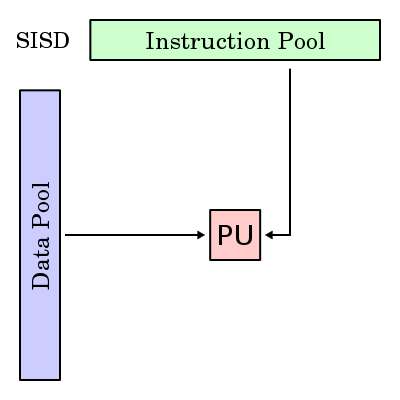
\includegraphics[width=\textwidth]{SISD.png}\\
        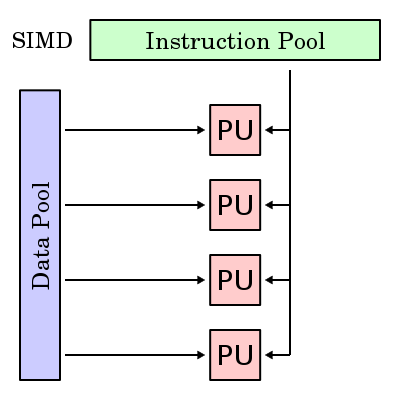
\includegraphics[width=\textwidth]{SIMD.png}
      \end{column}
      \begin{column}{.27\textwidth}
        \centering
        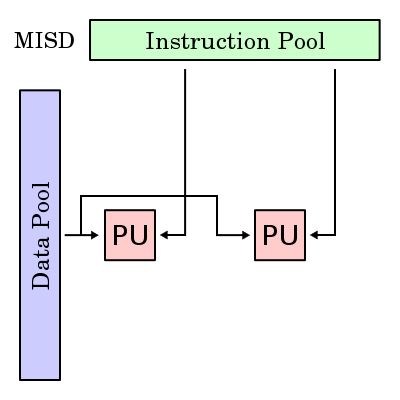
\includegraphics[width=\textwidth]{MISD.png}\\
        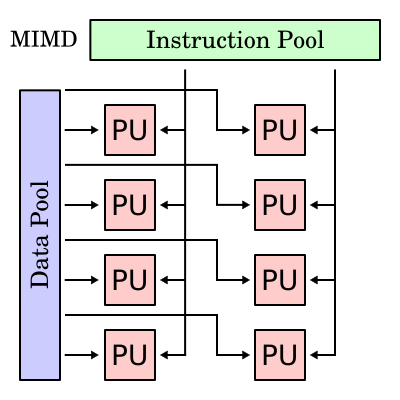
\includegraphics[width=\textwidth]{MIMD.png}
      \end{column}
    \end{columns}
    \hfill \tiny{\href{https://en.wikipedia.org/wiki/Flynn's\_taxonomy}{Flynn's~taxonomy}~by~Cburnett~/~\href{http://creativecommons.org/licenses/by-sa/3.0}{CC~BY~3.0}~/~presenting~the~four~together}

    \note{
      \begin{itemize}
        \item ask students to give examples of each
          \begin{itemize}
            \item SISD
              \begin{itemize}
                \item serial computer
              \end{itemize}
            \item SIMD
              \begin{itemize}
                \item gpu
                \item some modern cpus have simd extensions
              \end{itemize}
            \item MISD
              \begin{itemize}
                \item fault tolerance
              \end{itemize}
            \item MIMD (in many cases, this is further divided into a category
              commonly known as SPMD, single program multiple data)
              \begin{itemize}
                \item most common type of parallel computer (multi-thread or
                  multi-node)
              \end{itemize}
          \end{itemize}
        \item which of these might be interesting to us, i.e., which might make
          good parallel systems?
      \end{itemize}
    }
  \end{frame}

  \begin{frame}[c]{simd}
    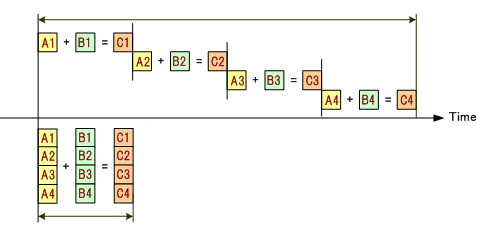
\includegraphics[width=\textwidth]{simd-execution.png}\\
    \hfill \tiny{\href{https://www.softek.co.jp/SPG/Pgi/TIPS/public/general/multicore-para.html}{SIMD}~/~cropped~from~original}

    \note{
      \begin{itemize}
        \item cuda / opencl are languages to express this type of parallelism,
          but we will not be studying them
        \item what sorts of problems might this be good for?
          \begin{itemize}
            \item matrix-oriented scientific computing
            \item media-oriented image and sound processors
          \end{itemize}
        \item simd is simpler and more energy efficient than mimd, why?
          \begin{itemize}
            \item only needs to fetch one instruction per ``cycle''
          \end{itemize}
        \item what would the mimd time line look like?
        \item so then what are the (dis)advantages of each of the
          classifications?
          \begin{itemize}
            \item simd works in lock stop, so does not require synchronization,
              which can make it easier to reason about
            \item mimd processing elements are autonomous, so can solve more
              complex problems
          \end{itemize}
      \end{itemize}
    }
  \end{frame}

  \begin{frame}{communication models}
    \begin{columns}
      \begin{column}{.48\textwidth}
        \begin{itemize}
          \item shared-address space
            \begin{itemize}
              \item UMA / NUMA / ccNUMA
            \end{itemize}
        \end{itemize}
      \end{column}
      \begin{column}{.48\textwidth}
        \begin{itemize}
          \item message-passing
        \end{itemize}
      \end{column}
    \end{columns}
    \vspace{3ex}
    \centering
    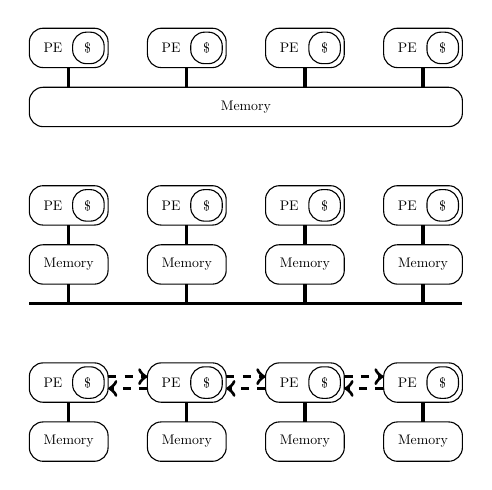
\begin{tikzpicture}[scale=.5,every node/.style={transform shape}]
      \foreach \x in {0,3,6,9}
      {
        \draw[very thick] ({\x+1},1) -- ({\x+1},1.5);
        \draw[rounded corners=5pt] (\x,1.5) rectangle ++(2,1);
        \node at ({\x+.6},2) {PE};
        \only<2>{\draw[rounded corners=5pt] ({\x+1.1},1.6) rectangle ++(.8,.8);}
        \only<2>{\node at ({\x+1.5},2) {\$};}
      }
      \draw[rounded corners=5pt] (0,0) rectangle ++(11,1);
      \node at (5.5,.5) {Memory};

      \foreach \x in {0,3,6,9}
      {
        \draw[rounded corners=5pt] (\x,-2.5) rectangle ++(2,1);
        \node at ({\x+.6},-2) {PE};
        \only<2>{\draw[rounded corners=5pt] ({\x+1.1},-2.4) rectangle ++(.8,.8);}
        \only<2>{\node at ({\x+1.5},-2) {\$};}
        \draw[very thick] ({\x+1},-3) -- ({\x+1},-2.5);
        \draw[rounded corners=5pt] (\x,-4) rectangle ++(2,1);
        \node at ({\x+1},-3.5) {Memory};
        \draw[very thick] ({\x+1},-4) -- ({\x+1},-4.5);
      }
      \draw[very thick] (0,-4.5) -- (11,-4.5);

      \foreach \x in {0,3,6,9}
      {
        \draw[rounded corners=5pt] (\x,-7) rectangle ++(2,1);
        \node at ({\x+.6},-6.5) {PE};
        \only<2>{\draw[rounded corners=5pt] ({\x+1.1},-6.9) rectangle ++(.8,.8);}
        \only<2>{\node at ({\x+1.5},-6.5) {\$};}

        \draw[very thick] ({\x+1},-7.5) -- ({\x+1},-7);
        \draw[rounded corners=5pt] (\x,-8.5) rectangle ++(2,1);
        \node at ({\x+1},-8) {Memory};
      }
      \foreach \u/\v in {2/3,5/6,8/9}
      {
        \draw[very thick,dashed,->] (\u,-6.35) -- (\v,-6.35);
        \draw[very thick,dashed,->] (\v,-6.65) -- (\u,-6.65);
      }
    \end{tikzpicture}

    \note{
      \begin{itemize}
        \item how do processing elements communicate with each other
          \begin{itemize}
            \item shared-address space
              \begin{itemize}
                \item everyone has access to everyone else's data
                \item communicate through shared memory
              \end{itemize}
            \item message-passing
              \begin{itemize}
                \item communicate through messages sent between PEs
                \item build on two basic operations, \emph{send} and
                  \emph{receive}
              \end{itemize}
          \end{itemize}
        \item why not just make everything uma?
        \item is there anything missing from this model?
          \begin{itemize}
            \item what is a cache for?
          \end{itemize}
        \item the existence of caches means that data can exist in multiple
          places
          \begin{itemize}
            \item a cache coherence protocol is required to ensure proper
              semantics and correct program execution
            \item have students think of a sequence of operations that would be
              incorrect without cache coherence
          \end{itemize}
      \end{itemize}
    }
  \end{frame}

  \begin{frame}{cache coherence}
      \begin{columns}
        \begin{column}{.52\textwidth}
          \begin{itemize}
            \item update
              \begin{itemize}
                \item increases communication on the bus
              \end{itemize}
          \end{itemize}
        \end{column}
        \begin{column}{.44\textwidth}
          \begin{itemize}
          \item invalidate
            \begin{itemize}
              \item increases idling time
            \end{itemize}
        \end{itemize}
      \end{column}
    \end{columns}

    \centering
    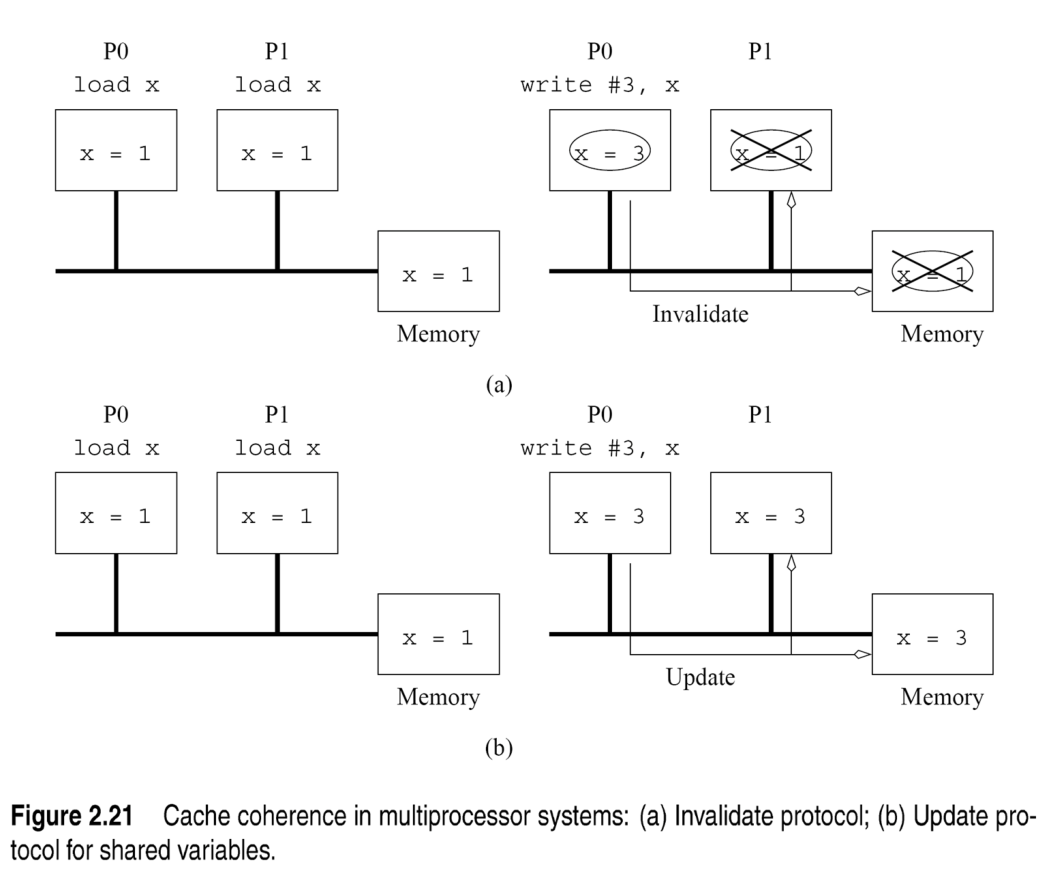
\includegraphics[width=.60\textwidth]{cc_protocols.pdf}\\
    \hfill \tiny{\href{}{}}

    \note{
      \begin{itemize}
        \item why is cache coherence important?
          \begin{itemize}
            \item maintains serializability --- just like ILP
          \end{itemize}
      \end{itemize}
      \begin{itemize}
        \item considerations for each of the two protocols
          \begin{itemize}
            \item update increases communication because a message is sent every
              time that a PE updates a value that it has in cache --- contrast
              this with invalidate which sends a single invalidate after the
              first update, but no subsequent messages
            \item invalidate increases idle time because whenever a PE accesses
              a value that has been invalidated, it must wait while the updated
              value is fetched --- contrast this with update, where the updated
              value would have been sent at the time of the update
          \end{itemize}
        \end{itemize}
      \begin{itemize}
        \item which do you think most processors use?
          \begin{itemize}
            \item invalidate
          \end{itemize}
      \end{itemize}
    }
  \end{frame}

  \begin{frame}{false sharing}
    \vspace{3ex}
    \centering
    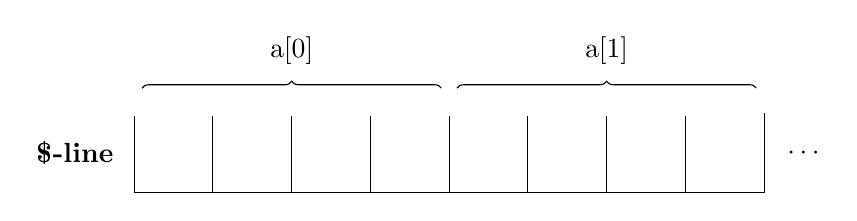
\begin{tikzpicture}
      \node at (-.75,4.5) {\textbf{\$-line}};
      \foreach \x in {0,...,7}
        \draw (\x,4) rectangle ++(1,1);
      \draw[white, ultra thick] (0,5) -- ++(8,0);
      \draw[decoration={brace,raise=-5pt},decorate] (0.1,5.5) --
        node[above] {a[0]} ++(3.8,0);
      \draw[decoration={brace,raise=-5pt},decorate] (4.1,5.5) --
        node[above] {a[1]} ++(3.8,0);
      \node at (8.5,4.5) {$\boldsymbol{\cdots}$};
    \end{tikzpicture}

    \begin{tabular}{lll}
      & \multicolumn{1}{c}{PE0} & \multicolumn{1}{c}{PE1}\\
      \multicolumn{1}{c}{time} & a[0] = 1 & a[1] = 7\\
      \multicolumn{1}{c}{\multirow{2}{*}{\Big\downarrow}} & a[0] = 2 & a[1] = 8\\
      & a[0] = 3 & a[1] = 9
    \end{tabular}

    \note{
      \begin{itemize}
        \item a few more notes about caches
        \begin{itemize}
          \item data is fetched from memory at the granularity of a cache line
          \item cache lines are fixed size (typically 64 bytes)
        \end{itemize}
      \end{itemize}
      \begin{itemize}
        \item consider this example
          \begin{itemize}
            \item what would happen if we were using invalidate protocol?
            \item remember, the cache line is copied into the cache of PE0
              \emph{and} PE1
            \item how can this be avoided?
          \end{itemize}
      \end{itemize}
    }
  \end{frame}

  %\begin{frame}[standout]
  %  \ifnotes
  %    \usebeamercolor[white]{normal text} % override bug fix in preamble
  %  \fi
  %\end{frame}

  \appendix

  \begin{frame}[c]
    \begin{center}\ccbysa\end{center}

    except where otherwise noted, this worked is licensed under
    \href{http://creativecommons.org/licenses/by-sa/4.0/}{creative commons
    attribution-sharealike 4.0 international license}
  \end{frame}
\end{document}
